\documentclass[journal]{IEEEtran}

\usepackage{amsthm}
\usepackage{float}
\usepackage{cite}										
\usepackage{amsmath}									
\usepackage{graphicx}
\usepackage{epstopdf}
\usepackage{float}
\usepackage{bm,upgreek}
\usepackage{amsfonts}
\usepackage{enumitem}
\usepackage{mathtools}
\usepackage{multirow}
\usepackage{booktabs}
\usepackage[subnum]{cases}
\usepackage{setspace}
\usepackage{color}
\usepackage{blkarray, bigstrut} 
\usepackage[caption=false,labelformat=simple]{subfig}
\renewcommand{\thesubfigure}{(\alph{subfigure})}
\pagenumbering{gobble}
\usepackage{xcolor}
\usepackage{pgfplots}
\pgfplotsset{compat=1.5}
\usepackage{pgfplotstable}
\usepgfplotslibrary{statistics}
\pgfplotsset{grid style={dotted,gray}}
\usepackage{tikz}
\usepackage{hyperref}

\usepackage{mathtools,nccmath}
\usepackage[ruled]{algorithm}
\usepackage{algpseudocode,algorithmicx}

\algnewcommand{\LineComment}[1]{\State \(\#\) #1}

\allowdisplaybreaks

\ifCLASSINFOpdf
\else
\fi
\hyphenation{op-tical net-works semi-conduc-tor}

\newcommand\tab[1][1cm]{\hspace*{#1}}

\pgfplotsset{legend image with text/.style={legend image code/.code={%
\node[anchor=west, align=right] at (0.0cm,0cm) {#1};}},}
\newenvironment{itemizeReduced}{
\begin{list}{}{\leftmargin=0em}
\setlength{\itemsep}{1pt}
\setlength{\parskip}{0pt}
\setlength{\parsep}{0pt}}{\end{list}
}

\makeatletter
\def\myline{\pgfutil@ifnextchar[{\my@line}{\my@line[]}}%
\def\my@line[#1](#2)(#3){%
\tikz[overlay] \draw[#1]  (#2)--(#3); 
}%
\algrenewcommand\algorithmicindent{1.0em}%

\newtheorem{example}{Example}

  \newcommand\xqed[1]{%
  \leavevmode\unskip\penalty9999 \hbox{}\nobreak\hfill
  \quad\hbox{#1}}
\newcommand\demo{\xqed{$\triangle$}}

\makeatletter
\renewcommand{\ALG@beginalgorithmic}{\small}
\makeatother

\makeatletter
\newcommand{\algrule}[1][.2pt]{\par\vskip.5\baselineskip\hrule height #1\par\vskip.5\baselineskip}
\makeatother

\usepackage{etoolbox}% http://ctan.org/pkg/etoolbox
\BeforeBeginEnvironment{algorithmic}{\kern 0.3\baselineskip}% Space above algorithmic environment
\AfterEndEnvironment{algorithmic}{\kern -0.1\baselineskip}% Space below algorithmic environment

%\usepackage[keeplastbox]{flushend}
\newtheorem{theorem}{Theorem}
\newtheorem{corollary}{Corollary} 
\newtheorem{definition}{Definition}
\newtheorem{remark}{Remark}


\makeatletter
\renewcommand{\ALG@beginalgorithmic}{\footnotesize}
\makeatother


\pgfplotsset{
    box plot/.style={
        /pgfplots/.cd,
        black,
        only marks,
        mark=-,
        mark size=\pgfkeysvalueof{/pgfplots/box plot width},
        /pgfplots/error bars/y dir=plus,
        /pgfplots/error bars/y explicit,
        /pgfplots/table/x index=\pgfkeysvalueof{/pgfplots/box plot x index},
    },
    box plot box/.style={
        /pgfplots/error bars/draw error bar/.code 2 args={%
            \draw  ##1 -- ++(\pgfkeysvalueof{/pgfplots/box plot width},0pt) |- ##2 -- ++(-\pgfkeysvalueof{/pgfplots/box plot width},0pt) |- ##1 -- cycle;
        },
        /pgfplots/table/.cd,
        y index=\pgfkeysvalueof{/pgfplots/box plot box top index},
        y error expr={
            \thisrowno{\pgfkeysvalueof{/pgfplots/box plot box bottom index}}
            - \thisrowno{\pgfkeysvalueof{/pgfplots/box plot box top index}}
        },
        /pgfplots/box plot
    },
    box plot top whisker/.style={
        /pgfplots/error bars/draw error bar/.code 2 args={%
            \pgfkeysgetvalue{/pgfplots/error bars/error mark}%
            {\pgfplotserrorbarsmark}%
            \pgfkeysgetvalue{/pgfplots/error bars/error mark options}%
            {\pgfplotserrorbarsmarkopts}%
            \path ##1 -- ##2;
        },
        /pgfplots/table/.cd,
        y index=\pgfkeysvalueof{/pgfplots/box plot whisker top index},
        y error expr={
            \thisrowno{\pgfkeysvalueof{/pgfplots/box plot box top index}}
            - \thisrowno{\pgfkeysvalueof{/pgfplots/box plot whisker top index}}
        },
        /pgfplots/box plot
    },
    box plot bottom whisker/.style={
        /pgfplots/error bars/draw error bar/.code 2 args={%
            \pgfkeysgetvalue{/pgfplots/error bars/error mark}%
            {\pgfplotserrorbarsmark}%
            \pgfkeysgetvalue{/pgfplots/error bars/error mark options}%
            {\pgfplotserrorbarsmarkopts}%
            \path ##1 -- ##2;
        },
        /pgfplots/table/.cd,
        y index=\pgfkeysvalueof{/pgfplots/box plot whisker bottom index},
        y error expr={
            \thisrowno{\pgfkeysvalueof{/pgfplots/box plot box bottom index}}
            - \thisrowno{\pgfkeysvalueof{/pgfplots/box plot whisker bottom index}}
        },
        /pgfplots/box plot
    },
    box plot median/.style={
        /pgfplots/box plot,
        /pgfplots/table/y index=\pgfkeysvalueof{/pgfplots/box plot median index},
        semithick,black
    },
    box plot width/.initial=1em,
    box plot x index/.initial=0,
    box plot median index/.initial=1,
    box plot box top index/.initial=2,
    box plot box bottom index/.initial=3,
    box plot whisker top index/.initial=4,
    box plot whisker bottom index/.initial=5,
}

\newcommand{\boxplot}[2][]{
    \addplot [box plot median,#1] table {#2};
    \addplot [forget plot, box plot box,#1] table {#2};
    \addplot [forget plot, box plot top whisker,#1] table {#2};
    \addplot [forget plot, box plot bottom whisker,#1] table {#2};
}

\pgfplotsset{compat=1.11, 
    /pgfplots/ybar legend/.style={
    /pgfplots/legend image code/.code={%
       \draw[##1,/tikz/.cd,yshift=-0.25em]
        (0cm,0cm) rectangle (6pt,0.8em);},
   },
}

\algnewcommand\algorithmicforeach{\textbf{for each}}
\algdef{S}[FOR]{ForEach}[1]{\algorithmicforeach\ #1\ \algorithmicdo}

\definecolor{black}{RGB}{50, 50, 50}
\definecolor{richburgundy}{RGB}{105, 36, 47}
\definecolor{steelblue}{RGB}{70, 98, 119}
\definecolor{forestgreen}{RGB}{46, 78, 49}
\definecolor{goldenrod}{RGB}{153, 116, 56}
\definecolor{rosybrown}{RGB}{133, 94, 84}


\begin{document}

\newlist{myitemize}{itemize}{3}
\setlist[myitemize,1]{label=\textbullet,leftmargin=6.5mm}

\title{JuliaGrid: An Open-Source Julia-Based Framework for Power System State Estimation}

\author{Mirsad~Cosovic,
        Ognjen~Kundacina,
        Muhamed~Delalic,
        Armin~Teskeredzic,
        Darijo~Raca,
        Amer~Mesanovic,
        Dragisa~Miskovic,
        Dejan Vukobratovic,
        Antonello Monti% <-this % stops a space

\thanks{M. Cosovic is with Faculty of Electrical Engineering, University of Sarajevo, Bosnia and Herzegovina, and the Institute for Artificial Intelligence Research and Development of Serbia (e-mail: mcosovic@etf.unsa.ba); O. Kundacina and D. Miskovic are with the Institute for Artificial Intelligence Research and Development of Serbia (e-mail: ognjen.kundacina@ivi.ac.rs, dragisa.miskovic@ivi.ac.rs); M. Delalic and D. Raca are with Faculty of Electrical Engineering, University of Sarajevo, Bosnia and Herzegovina (e-mail: muha.delalic@gmail.com, draca@etf.unsa.ba); A. Teskeredzic is with Institute for Automation of Complex Power Systems, E.ON Energy Research Center, RWTH Aachen University, Germany (e-mail: armin.teskeredzic@eonerc.rwth-aachen.de), A. Mesanovic is with Siemens AG, Munich, Germany (email: amer.mesanovic@siemens.com); D. Vukobratovic is with Faculty of Technical Sciences, University of Novi Sad, Serbia (email: dejanv@uns.ac.rs); A. Monti is with the Institute for Automation of Complex Power Systems, E.ON Energy Research Center, RWTH Aachen University, Germany, and with the Fraunhofer FIT, Aachen, Germany (e-mail: amonti@eonerc.rwth-aachen.de).}
\thanks{This paper has received funding from the European Union's Horizon 2020 research
and innovation staff exchange grant agreement number 101086387.}}

\markboth{}%
{Shell \MakeLowercase{\textit{et al.}}: Bare Demo of IEEEtran.cls for IEEE Journals}

\maketitle


\begin{abstract}
Modern electric power systems have an increasingly complex structure due to rise in power demand and integration of diverse energy sources. Monitoring these large-scale systems, which relies on efficient state estimation (SE), represents a challenging computational task and requires efficient simulation tools for power system steady-state analyses. Motivated by this observation, we propose JuliaGrid, an open-source framework written in the Julia programming language, designed for high performance execution across multiple platforms. The framework implements observability analysis, weighted least-squares and least-absolute value estimators, bad data analysis, and various algorithms related to phasor measurements. To complete power system analysis, the framework includes power flow and optimal power flow, enabling measurement generation for the SE routines. Leveraging computationally efficient algorithms, JuliaGrid solves large-scale systems across all SE routines with competitive execution times compared to other open-source frameworks. These capabilities are validated through simulations on power systems with 10\,000, 20\,000 and 70\,000 buses.
\end{abstract}


\begin{IEEEkeywords}
Observability Analysis, Optimal PMU Placement, State Estimation Algorithm, Bad Data Analysis, Power Flow, Optimal Power Flow, Large-Scale Power Systems, Open-Source, Julia 
\end{IEEEkeywords}

\IEEEpeerreviewmaketitle

\section{Introduction}
Electric power systems are a vital fabric of modern society, underpinning technological and industrial progress. Traditionally, these systems follow a hierarchical structure comprising generation, transmission, and consumption components, with power flowing from large producers to consumers. However, the increasing integration of renewable energy sources and the deregulation of power systems have resulted in more complex control, leading to a degradation in their optimal performance. Therefore, power systems monitoring becomes a key building block to enhance control and power flow efficiency. Reliable monitoring depends on computationally efficient and accurate state estimation (SE), which represents one of the fundamental components of modern energy management systems.

Supervisory control and data acquisition (SCADA) technology gathers input data for SE. SCADA provides the communication infrastructure to collect legacy measurements, including bus voltage magnitudes, bus active and reactive power injections, branch current magnitudes, and branch active and reactive power flows. Over the past few decades, the development of phasor measurement units (PMUs) enabled the measurement of bus voltage and branch current phasors with high accuracy and high sampling rates. PMUs have been instrumental in the development of wide-area measurement systems (WAMSs), which aim to provide real-time monitoring and control of power systems~\cite{gomez2011use}.

After collecting measurements at control centers, SE determines the present state of the power system, inherently defined by the known bus voltages~\cite[Sec.1.2]{abur}. The SE process involves four key routines: the network topology processor, observability analysis, SE algorithm, and bad data analysis. The network topology processor uses circuit breakers status information to form an energized network topology, creating a bus/branch model of the power system~\cite{sasson1973automatic}. Observability analysis discovers whether the underlying system of equations solved by SE algorithm has a unique solution (i.e., system is observable). If the system is unobservable, observability analysis requires additional measurements, known as pseudo-measurements. The analysis determines the minimal set of pseudo-measurements needed to make the system observable, ensuring a unique state estimate~\cite{monticelli1985network}. SE algorithm obtains state estimate by filtering noise-induced and redundant measurements~\cite{schweppe1970exact}. Finally, bad data analysis identifies and eliminates measurement errors (i.e., outliers), followed by a new execution of SE algorithm~\cite{handschin1975bad}.

\subsection{Motivation}
The scale and complexity of power systems impact SE, driving extensive research efforts to develop new approaches and computationally efficient algorithms for handling all SE routines~\cite{korresDistributed, complexBP, cosovicBP, yilmaz, muscas2015multiarea, zargar2020multiarea}. In this context, a comprehensive framework enabling comparison of novel to the state-of-the-art algorithms, represents an invaluable resource. JuliaGrid addresses these needs by providing a complete solution: from artificially generating measurements based on power flow (PF), optimal power flow (OPF), or using real data, to determining optimal PMU placement. Moreover, JuliaGrid includes highly optimized and computationally efficient algorithms for observability analysis, SE algorithms, and bad data analysis, all tailored for large-scale power systems.

We host JuliaGrid on GitHub, one of the most popular platform for sharing and managing open-source code. In addition to code itself, we provide extensive documentation alongside the framework, which is available at the following 
\href{https://mcosovic.github.io/JuliaGrid.jl/stable/}{link}\footnote{\url{https://mcosovic.github.io/JuliaGrid.jl/stable/}}. The provided online documentation consists of manual, tutorials, examples, and API references. The manual outlines users how to use available functions, function and object signature, and provides instructions for various analysis types. The tutorials cover theoretical underpinnings of state-of-the-art algorithms and provide detailed explanation for all mathematical models. The examples provide a wide range of toy examples coupled with various power system datasets highlighting JuliaGrid's abilities in steady-state and quasi-steady-state analyses. Finally, API references list all objects, functions and methods within the package. This comprehensive documentation enhances the JuliaGrid's educational value, allowing both students and researchers to develop an in-depth understanding of mathematical models and their practical implementation within power system steady-state analyses.

\subsection{Open-Source Steady-State Power System Frameworks}
Over the past three decades, open-source power system frameworks gained significant popularity and availability, resulting in the creation of numerous advanced simulation frameworks~\cite{groissbock2019open}. One of the earliest and the most significant framework in this domain is {\scalebox{0.85}{MATPOWER}}~\cite{zimmerman2010matpower}, which has greatly influenced both education and research communities due to its well-structured and easily understandable open-source {\scalebox{0.85}{MATLAB}} code. {\scalebox{0.85}{MATPOWER}} excels in solving PF and OPF problems, and includes an optimal scheduling feature for market simulations~\cite{zimmerman2013matpower}. Despite its strengths, {\scalebox{0.85}{MATPOWER}}'s key limitation lies in its dependence on commercial software platform. The issue is addressed by {\scalebox{0.85}{PYPOWER}}~\cite{lincoln2011learning}, a Python-based adaptation of {\scalebox{0.85}{MATPOWER}}, which serves as a complete open-source alternative. More recently, pandapower adopted the {\scalebox{0.85}{PYPOWER}} framework, focusing on the automation of quasi-steady-state analysis and optimization for balanced three-phase power systems. Unlike {\scalebox{0.85}{MATPOWER}} and {\scalebox{0.85}{PYPOWER}}, pandapower allows users to define power systems using nameplate parameters, further enhancing its utility and flexibility~\cite{thurner2018pandapower}. {\scalebox{0.85}{PSAT}} and PowSyBl represent frameworks based on {\scalebox{0.85}{MATLAB}}/Simulink and Python/Java, respectively, supporting PF, OPF, and time-domain simulations, making it a versatile resource for power system analysis~\cite{milano2005open}.

In addition to frameworks based on {\scalebox{0.85}{MATLAB}} and Python, OpenDSS, GridLAB-D, and PowerModels represent frameworks with inherent educational and research purposes based on Delphi, C/C++, and Julia programming languages, respectively. OpenDSS offers a wide range of functionalities, primarily focused on distribution systems and distributed energy resources~\cite{dugan2011open}. GridLAB-D is an advanced tool for static simulations using agent-based models~\cite{chassin2008gridlab}. PowerModels is an open-source framework designed for solving PF and OPF problems, leveraging just-in-time compilation to enhance performances~\cite{coffrin2018powermodels}. Finally, OpenModelica represents a general purpose framework supporting power system analyses through different third-party packages such as PowerGrids and PowerSystems~\cite{openmodelica, franke2014flexible}.

Among the primary steady-state analyses, SE has received comparatively less attention than PF and OPF, which have dominated most research efforts. Pandapower is one of the first to address this gap by introducing SE routines, including nonlinear SE using legacy measurements with weighted least-squares (WLS), robust WLS, and least-absolute value (LAV) estimators, along with bad data analysis. However, pandapower lacks observability analysis, integration of PMUs in various coordinate systems, and algorithms related to PMUs, such as linear SE using phasor measurements only. Next, PowerGridModel, implemented in Python and C, supports SE for distribution power systems and observability analysis, missing the rest of the SE routines~\cite{PowerGridModel}. 

Recent efforts tried to address some of these missing features, with authors developing educational tools for SE in power systems using Python~\cite{do2022educational}. While this tool is excellent for educational purposes, it lacks several key SE algorithms. For example, more robust WLS methods for handling ill-conditioned cases and the implementation of a LAV estimator are missing. Additionally, there is a need for more efficient implementations of existing algorithms to support large-scale analysis, like the use of sparse inverse techniques for bad data analysis. Furthermore, the framework does not account for phase-shifting transformers, limiting its applicability to standardized power system data, such as those used in IEEE test cases. While PMUs integration into SE models is possible (unlike in pandapower), the framework lacks the ability to handle PMUs in different coordinate systems. 

To the best of our knowledge, JuliaGrid is the first open-source framework designed to meet these requirements by providing state-of-the-art SE routines, optimized for large-scale power systems. Following subsection outlines key design principles and architecture underpinning JuliaGrid framework illustrating its educational and research-oriented objectives. 

\subsection{Overview of JuliaGrid Features}
JuliaGrid is implemented in the Julia programming language, utilizing just-in-time compilation to enhance performance and ensure cross-platform compatibility. The framework's architecture follows a code-reusability paradigm, allowing users to easily customize their experiments. For example, modifying the power system topology or adjusting measurements trigger an update of the existing vectors and matrices without rebuilding them from scratch, thus facilitating computationally fast and efficient steady-state and especially quasi-steady-state analysis. 

In JuliaGrid, users have access to different types of analyses using the AC or DC models, where DC model is obtained by the linearization of the AC model resulting in an approximate solution. Following this approach, JuliaGrid integrates PF and OPF analyses for both models, enabling users to efficiently generate measurement data. Once the measurement data is generated, the framework provides the following capabilities:

\vspace{1mm}
\noindent {Observability Analysis}  
\begin{itemize}[leftmargin=*] 
    \item Identify flow or maximal observable islands.  
    \item Restore observability using pseudo-measurements.  
    \item Identify optimal PMU locations to enhance observability.  
\end{itemize}

\vspace{1mm}
\noindent {State Estimation Models}  
\begin{itemize}[label=\textbullet, leftmargin=*] 
    \item Build nonlinear SE model using legacy and/or phasor measurements, with phasors represented in either polar or rectangular coordinates, optionally considering covariances.
    \item Build linear SE model using PMUs only, with optional inclusion of covariances. 
    \item Build DC state estimation (DCSE) model.  
\end{itemize}  

\vspace{1mm}
\noindent {State Estimation Algorithms}  
\begin{itemize}[label=\textbullet, leftmargin=*] 
    \item Solve SE models to obtain the WLS estimators.  
    \item Employ robust WLS formulation for numerical stability.  
    \item Solve SE models to obtain the LAV estimators.  
\end{itemize}  

\vspace{1mm}
\noindent {Bad Data Analysis}  
\begin{itemize}[label=\textbullet, leftmargin=*] 
    \item Analyze measurement residuals to detect outliers.  
    \item Remove outliers from SE models.  
\end{itemize}  

JuliaGrid provides a comprehensive framework combining heterogeneous models analysis, allowing access to all intermediate results during analysis. More precisely, power system model and measurement data are represented as the objects. Once created, these objects can be modified, updated or passed to different type of analyses. Furthermore, each of the analyses represent an independent object, which can be modified and updated. These features are implemented through built-in functions facilitating straightforward and streamlined workflow. As a consequence, this design allows users to execute and compare results from different analyses during the same runtime, resulting in simple and intuitive analysis of the quasi-steady-state conditions. The object-oriented paradigm empowers users to access vectors, matrices, and factorized matrices at each step by decomposing PF and WLS SE algorithms. This granular control is complemented by the ability to choose different factorization methods, such as LDL, LU, or QR, enabling users to customize the solution process for specific performance goals or application requirements. Building on this foundation, JuliaGrid integrates the OPF and LAV SE algorithms using the JuMP package~\cite{Lubin2023}, a domain-specific modeling language for mathematical optimization. Renowned in the research community for its versatility, JuMP enables JuliaGrid to run a wide range of optimization solvers (e.g., Ipopt and Gurobi) for tackling large-scale systems. To enhance the ability to adapt and refine models as needed, JuliaGrid facilitates the seamless extension of OPF models, allowing users to add, update, or remove optimization variables and constraints without rebuilding the model. At the same time, users retain access to vectors and matrices for in-depth examination and analysis. 

JuliaGrid core design principle resolves around support for large-scale analysis, employing computationally efficient algorithms. For example, JuliaGrid leverages Julia's column-major order for storing multidimensional arrays, by constructing matrices through accessing columns during all analyses. This strategy minimizes memory access overhead and improves cache efficiency, by aligning operations with the underlying memory layout. As a result, users experience faster data retrieval and more efficient computations, particularly for large-scale analysis. Additionally, JuliaGrid supports multiple unit systems for input data and offers flexible options for printing and exporting results, ensuring tailored outputs conforming to specific needs and preferences of individual users. 

In the following sections, beside theoretical background of state-of-the-art power system steady-state modeling and related analyses, we outline framework's key implementation design choices ensuring high computational efficiency as illustrated in performance evaluation section. 

\section{Steady-State Power System Models}
A common approach to describing power system network topology is the bus/branch model, represented by a graph $\mathcal{G} = (\mathcal{N}, \mathcal{E})$. The set of nodes $\mathcal{N} = \{1, \dots, n\}$ corresponds to buses, while the set of edges $\mathcal{E} \subseteq \mathcal{N} \times \mathcal{N}$ represents the branches of the power system. Each branch is described using a two-port $\pi$-model, resulting in the unified branch model, illustrated in Fig. \ref{fig:pi_model}. The unified branch model is characterized by its series admittance $y_{ij}$, shunt admittance $y_{\mathrm{s}ij}$, and transformer complex ratio $\alpha_{ij}$, where $(i, j) \in \mathcal{E}$.

\begin{figure}[ht]
    \centering
    \includegraphics[width=8.5cm]{./figure/pi_model.eps}
    \caption{The unified branch model for modeling transmission lines, in-phase transformers, and phase-shifting transformers.}
    \label{fig:pi_model}
\end{figure}   

The series admittance $y_{ij}$ is defined as the reciprocal of the series impedance $z_{ij} = r_{ij} + \mathrm{j}x_{ij}$, where $r_{ij}$ represents the resistance and $x_{ij}$ is the reactance of the branch. The shunt admittances are given by $y_{\mathrm{s}ij} = g_{\mathrm{s}ij} + \mathrm{j}b_{\mathrm{s}ij}$, where $g_{\mathrm{s}ij}$ is the shunt conductance and $b_{\mathrm{s}ij}$ is the shunt susceptance. Both of these parameters take positive values for real transmission lines. The shunt conductance $g_{\mathrm{s}ij}$, often negligibly small, can be omitted in many cases. However, we retain the flexibility to include $g_{\mathrm{s}ij}$ in the model.

The transformer complex ratio is defined as $\alpha_{ij} = \tau_{ij}^{-1}e^{-\text{j}\phi_{ij}}$, where $\tau_{ij} \neq 0$ is the off-nominal transformer turns ratio, while $\phi_{ij}$ is the transformer phase shift angle. The primary side of the transformer is always considered to be connected to the $i \in \mathcal{N}$ bus of the branch $(i, j) \in \mathcal{E}$. Therefore, the admittance $y_{ij}$ is specified on the secondary side of the transformer. This distinction is important because JuliaGrid allows the definition of branch parameters not only in per-unit values but also in ohms and siemens.

To summarize, for $\tau_{ij} = 1$ and $\phi_{ij} = 0$, the unified model represents a transmission line. In-phase transformers are defined for $\tau_{ij} \neq 1$, $\phi_{ij} = 0$, and $y_{\mathrm{s}ij} = 0$, while phase-shifting transformers are characterized by $\tau_{ij} \neq 1$, $\phi_{ij} \neq 0$, and $y_{\mathrm{s}ij} = 0$.

In addition to these parameters, power systems may include capacitor banks or inductors for reactive power compensation. Depending on the analysis requirements, additional data, such as generator outputs and power demands at buses, can be incorporated into the model. To load power system data, JuliaGrid provides diverse input options, accommodating various user requirements. Users can either construct data from scratch using built-in functions, import it from {\scalebox{0.85}{MATPOWER}} case files, or load models from the hierarchical data format version 5 (HDF5). The HDF5 format is an open-source standard excelling at managing large and heterogeneous datasets. Because of its efficient data handling and rapid loading capabilities, HDF5 is well-suited for large-scale power systems. JuliaGrid eases the use of this format by offering a built-in function to save constructed power system data as HDF5 file, facilitating its future reuse and supporting streamlined workflows with improved performance.

\subsection{AC Model}
We use the AC model, a fundamental component of our framework, to analyze power systems without approximations. Using Kirchhoff's circuit laws, the unified branch model can be described by the following complex expression:
\begin{equation}
  \begin{bmatrix}
    \bar{I}_{ij} \\ \bar{I}_{ji}
  \end{bmatrix} =
  \begin{bmatrix}
    \cfrac{1}{\tau_{ij}^2}({y}_{ij} + y_{\text{s}ij}) & -\alpha_{ij}^*{y}_{ij}\\
    -\alpha_{ij}{y}_{ij} & {y}_{ij} + y_{\text{s}ij}
  \end{bmatrix}
  \begin{bmatrix}
    \bar{V}_i \\ \bar{V}_j
  \end{bmatrix},
  \label{ACPiModel}
\end{equation}
where $\bar{I}_{ij}$ and $\bar{I}_{ji}$, $(i,j) \in \mathcal{E}$, represent the complex currents at the two sides of the branch, while $\bar{V}_i$ and $\bar{V}_j$ represent the complex bus voltages at buses $i \in \mathcal{N}$ and $j \in \mathcal{N}$, respectively.

As a result, derivation of all equations used in JuliaGrid related to the AC model follows from \eqref{ACPiModel}. These include equations for active and reactive power flows and injections, current magnitudes and angles in both polar and rectangular coordinate systems, as well as the real and imaginary components of the currents.

\subsection{DC Model}
The DC model is derived by linearizing the AC model defined by~\eqref{ACPiModel}. For high-voltage transmission networks under steady-state operating conditions, the voltage angle difference between adjacent buses $(i,j) \in \mathcal{E}$ is negligible $(\theta_{i}-\theta_{j} \approx 0)$, implying $\cos (\theta_{i}-\theta_{j})\approx 1$ and $\sin (\theta_{i}-\theta_{j}) \approx \theta_{i}-\theta_{j}$. Additionally, all bus voltage magnitudes are approximately $V_i \approx 1$, $i \in \mathcal{N}$, while branch series resistances and shunt admittances are neglected. As a result, the DC model disregards reactive powers and transmission losses, accounting only for active powers. Based on these assumptions and using \eqref{ACPiModel}, the following is obtained:
\begin{equation}
  \begin{bmatrix}
    P_{ij} \\ P_{ji}
  \end{bmatrix} = \cfrac{1}{\tau_{ij}x_{ij}}
  \begin{bmatrix*}[r]
    1 && -1\\
    -1 && 1
  \end{bmatrix*}
  \begin{bmatrix}
    \theta_{i} \\ \theta_{j}
  \end{bmatrix} + \cfrac{\phi_{ij}}{\tau_{ij}x_{ij}}
  \begin{bmatrix*}[r]
    -1 \\ 1
  \end{bmatrix*},
  \label{DCPiModel}
\end{equation}
where $P_{ij}$ and $P_{ji}$, $(i,j) \in \mathcal{E}$, represent the active power flows at the two sides of the branch, while $\theta_i$ and $\theta_j$ represent the bus voltage angles at buses $i \in \mathcal{N}$ and $j \in \mathcal{N}$, respectively. All DC analyses performed in JuliaGrid are based on the equations derived from \eqref{DCPiModel}.

\section{Power Flow and Optimal Power Flow}
The primary motivation for providing PF and OPF analyses is to support SE as a data source for generating measurements. Furthermore, these analyses follow JuliaGrid's core design principle offering a high degree of customization. This principle allows these analyses to be used independently of the SE routines.

\subsection{Power Flow}
JuliaGrid supports both AC power flow (ACPF) and DC power flow (DCPF) analyses. For ACPF, we implement solvers based on the Newton-Raphson method~\cite{tinney1967power}, the fast Newton-Raphson method with XB and BX formulations~\cite{van1989general}, and the Gauss-Seidel method~\cite{glimn1957automatic}. JuliaGrid allows users to update parameters for buses, branches, and generators, supports the addition of new branches and generators, without recreating vectors and matrices related to AC and DC models from scratch. For example, once the nodal admittance matrices are set, changes in branch parameters or branch statuses (from in-service to out-of-service, and vice versa) simply require updating the stored matrices. These features allow for the effective execution of quasi-steady-state PF analyses.

In addition, for ACPF with the fast Newton-Raphson method and DCPF, JuliaGrid tracks changes in the vectors and matrices associated with these models. The framework reuses factorized matrices whenever possible, improving computational efficiency during quasi-steady-state analyses. To illustrate, modifications to generator outputs and/or load parameters represent ideal scenario, significantly reducing the computational burden. To complement these features, JuliaGrid tracks the pattern of nonzero elements in the coefficient matrix of the DCPF, together with the Jacobian matrices used in the Newton-Raphson and fast Newton-Raphson methods. This tracking enables in-place factorization of these matrices, reducing the number of memory allocations.

\subsection{Optimal Power Flow}
The AC optimal power flow (ACOPF) and DC optimal power flow (DCOPF) analyses in JuliaGrid are built using the JuMP package, enabling intuitive manipulation and customization of these analyses. ACOPF focuses on minimizing an objective function related to the costs of generator active and reactive power outputs, while DCOPF considers only active power outputs~\cite{dommel1968optimal}. Similar to {\scalebox{0.85}{MATPOWER}}, these costs can be represented as polynomial or piecewise linear functions. For ACOPF, generator capability curves can be modeled accounting for a tradeoff between the active and reactive power outputs of the generators, adding flexibility to constraint modeling. To enable a warm start of the OPF, users can manually define initial primal values or use results from PF, as well as set initial dual values.

\section{Measurement Model}
Two primary technologies, SCADA and WAMS, gather measurements distributed across the power systems, contributing to the set of measurements $\mathcal{M}$.

Legacy measurements with low sampling rates, provided by SCADA, contributes to subsets of the set $\mathcal{M}$, each representing different types of measurements. These subsets include measurements for bus voltage magnitudes $\mathcal{V}$, branch current magnitudes $\mathcal{I}$, active power flows and injections $\mathcal{P}$, and reactive power flows and injections $\mathcal{Q}$. 

Furthermore, WAMS utilizes PMUs to provide high-sampling-rate data. While the single PMU typically measures the bus voltage phasor and the current phasors of all branches connected to the bus, we redefine this concept to offer greater flexibility. In JuliaGrid framework, a PMU measures individual phasors, either bus voltage or branch current, each characterized by magnitude, angle, and corresponding variances in the polar coordinate system. This approach extends the set $\mathcal{M}$ by including subsets $\bar{\mathcal{V}}$ for bus voltage phasors and $\bar{\mathcal{I}}$ for branch current phasors. These measurements can be included in SE models directly in polar coordinates, or alternatively by converting them into rectangular coordinates. Note that this inclusion can happen independently for each measurement, either in one or other coordinate system.

Each legacy measurement, as well as each magnitude and angle of phasor measurement, is associated with a measured value $z_i$, a measurement error $u_i \sim \mathcal{N} (0, v_i)$, where $v_i$ represents the variance, and a measurement function $h_i(\mathbf{x}_i)$. Here, $\mathbf{x}_i$ represents a subvector formed by selecting specific elements of the state variable vector $\mathbf{x} = [x_1, \dots, x_m]^{\mathrm{T}}$. The probability density function for the $i$-th measurement is proportional to:
\begin{equation}
  \mathcal{N}(z_i|\mathbf{x}_i,v_i) \propto \exp\Bigg\{-\cfrac{[z_i-h_i(\mathbf{x}_i)]^2}{2v_i}\Bigg\}.
  \label{gauss}
\end{equation}

In JuliaGrid the generation of measurement function $h_i(\mathbf{x}_i)$ follows the selection of SE model, and the function is derived from either \eqref{ACPiModel} or \eqref{DCPiModel}. The measurement value $z_i$ can be provided directly or alternatively generated artificially by adding white Gaussian noise $u_i$ to the exact value of the respective electrical quantity $e_i$, resulting in the measurement value $z_i = e_i + u_i$. 

To construct the measurement set $\mathcal{M}$, JuliaGrid provides built-in functions that use exact values obtained from ACPF or ACOPF analysis. Additionally, JuliaGrid implements the logic to randomize the availability of these measurements, allowing users to specify the number of in-service or out-of-service measurements for the entire set or within individual subsets. Also, users can randomize the number of in-service measurements by setting a redundancy value. In addition to these group manipulation functionalities, JuliaGrid supports options for adding, updating, or manipulating each individual measurement, also modifying SE models, thus allowing faster steady-state and quasi-steady-state analyses. Once the measurement model is constructed, the model can be saved in an HDF5 file for later use. 

Followed by definition of the measurement model based on the set $\mathcal{M}$, the relevant measurements can be selected to form the chosen SE model. For example, all measurements from the set $\mathcal{M}$ are included for the case of nonlinear SE, while the subsets of phasor measurements from $\mathcal{M}$ are used for linear SE with PMUs only. Therefore, depending on the selection of the SE model and the measurement set $\mathcal{M}$, the following system of equations can be formulated:
\begin{equation}
    \mathbf{z} = \mathbf{h}(\mathbf{x}) + \mathbf{u},
    \label{measurementModel}
\end{equation}
where $\mathbf{h}(\mathbf{x}) = [h_1(\mathbf{x}_1), \dots, h_k(\mathbf{x}_k)]^{\mathrm{T}}$ is the vector of measurement functions, $\mathbf{z} = [z_1, \dots, z_k]^{\mathrm{T}}$ is the vector of measurement values, and $\mathbf{u} = [u_1, \dots, u_k]^{\mathrm{T}}$ is the vector of measurement errors. The error vector $\mathbf{u}$ follows a zero-mean Gaussian distribution with a covariance matrix $\bm{\Sigma}$. The diagonal elements of $\bm{\Sigma}$ represent the measurement variances $\mathbf{v} = [v_1, \dots, v_k]^T$, while the off-diagonal elements correspond to the covariances between the measurement errors $\mathbf{w} = [w_1, \dots, w_k]^T$. These covariances arise only when phasor measurement functions are expressed in rectangular coordinates, which is supported by JuliaGrid. In many cases, however, these covariances are neglected~\cite{gomez2011use}, resulting in a diagonal covariance matrix $\bm{\Sigma}$.   

\section{Observability Analysis}
The SE algorithm aims to estimate the values of the state variables $\mathbf {x}$ based on the measurement model \eqref{measurementModel}. Prior to applying the SE algorithm, the observability analysis determines the existence and uniqueness of the solution for the system of equations \eqref{measurementModel}. For the cases where a unique solution is not guaranteed, the observability analysis identifies observable islands and adds set of equations defined by pseudo-measurements to achieve a unique solution~\cite{cosovic2021observability}.

In addition, JuliaGrid supports optimal PMU placement algorithm~\cite{gou2008optimal}, which identifies the minimum number of PMUs required to achieve observability. In other words, this functionality constructs a measurement model \eqref{measurementModel} that guarantees a unique solution.

\subsection{Identification of Observable Islands}
JuliaGrid utilizes standard observability analysis based on the linear decoupled measurement model~\cite{monticelli1985observability}, where active power measurements from the set $\mathcal{P}$ are used to estimate bus voltage angles, while reactive power measurements from the set $\mathcal{Q}$ are used to estimate bus voltage magnitudes. This approach assumes active and reactive power measurement pairs, allowing using only active power measurements for observability analysis. Additionally, JuliaGrid provides the option to include bus voltage phasor measurements from the set $\bar{\mathcal{V}}$, enhancing the functionality for more comprehensive observability analysis.

If the system is unobservable, the observability analysis must identify all potential observable islands that can be independently solved. In this context, JuliaGrid recognizes either flow or maximal observable islands. The choice between types of islands depends on the power system's structure and the available measurements. Opting to detect only flow observable islands simplifies the island detection procedure but increases the complexity of the observability restoration, compared to identifying maximal observable islands.

To identify flow observable islands, JuliaGrid employs a topological method outlined in~\cite{horisberger1985observability}. The process begins with the examination of all active power flow measurements, aiming to determine the largest sets of connected buses linked by branches with active power flow measurements. Subsequently, the analysis considers individual boundary or tie active power injection measurements, involving two islands that may potentially be merged into a single observable island. We extend the analysis with an additional processing step to identify maximal observable islands. After processing the individual injection tie measurements, we are left with a set of injection measurements unused in the previous step. We now examine these measurements for possible merging of flow islands~\cite{horisberger1985observability}.

\subsection{Observability Restoration}
After determining the islands, the observability restoration merges these islands in a manner that protects previously determined observable states from being altered by the new set of equations defined by the pseudo-measurements. This is accomplished by selecting a non-redundant subset of pseudo-measurements that augment the existing set of equations with linearly independent equations~\cite[Sec. 7.3.2]{monticelliBook}.

Following the island detection step, the power system is divided into $s$ islands. Next, we focus on the set of measurements $\mathcal{M}_\mathrm{r} \subset \mathcal{P} \cup \bar{\mathcal{V}}$, which consists solely of active power injection measurements at tie buses and bus voltage angle measurements. These measurements are retained from the step where observable islands are identified. Based on these measurements, we introduce the matrix $\mathbf{H}_\mathrm{r} \in \mathbb{R}^{r \times s}$, where $r = |\mathcal{M}_\mathrm{r}|$. This matrix represents the coefficient matrix of a reduced network, with $s$ columns corresponding to the islands and $r$ rows corresponding to the set $\mathcal{M}_\mathrm{r}$~\cite{korres2011gram, manousakis2010observability}.

The next step involves a new user-defined measurement model containing pseudo-measurements. From this set, the restoration process uses only the following measurements: active power flows between tie buses, active power injections at tie buses, and bus voltage angles. This subset of pseudo-measurements $\mathcal{M}_\mathbf{p}$ forms the reduced coefficient matrix $\mathbf{H}_\mathbf{p} \in \mathbb{R}^{p \times s}$, where $p = |\mathcal{M}_\mathbf{p}|$. Finally, we observe the coefficient matrix defined as:
\begin{equation}
  \mathbf H = \begin{bmatrix} \mathbf H_{\text{r}} \\ \mathbf H_{\text{p}} \end{bmatrix},
\end{equation}
and forms the corresponding Gram matrix:
\begin{equation}
  \mathbf D = \mathbf H \mathbf H^T.
\end{equation}
The decomposition of $\mathbf D$ into its $\mathbf Q$ and $\mathbf R$ factors is achieved through QR factorization. Measurements needed to ensure unique state estimate, are identified by the non-zero diagonal elements corresponding to pseudo-measurements in $\mathbf{R}$. Specifically, if a diagonal element satisfies $|R_{ii}| \ge \epsilon$, JuliaGrid designates the corresponding measurement as non-redundant, where $\epsilon$ represents a pre-determined zero pivot threshold. Finally, these pseudo-measurements from the set $\mathcal{M}_\mathbf{p}$ are transferred to the set of measurements $\mathcal{M}$ for further processing, such as running the nonlinear SE algorithm.

\subsection{Optimal PMU Placement}
The primary goal of PMU placement algorithm is to identify the minimal set of PMUs such that the entire system is observable. JuliaGrid utilizes the optimal PMU placement algorithm proposed in~\cite{gou2008optimal}. The optimal positioning of PMUs is framed as an integer linear programming problem:
\begin{equation}
  \begin{aligned}
    \text{minimize}& \;\;\; \sum_{i=1}^n d_i\\
    \text{subject\;to}& \;\;\; \sum_{j = 1}^n a_{ij}d_j \ge 1,\;\;\; i = 1,\dots,n,
  \end{aligned}
\end{equation} 
where $d_i \in \mathbb{F} = \{0,1\}$ is the PMU placement decision variable associated with bus $i \in \mathcal{N}$. The binary parameter $a_{ij} \in \mathbb{F}$ indicates the connectivity of the power system network, where $a_{ij}$ can be directly derived from the nodal admittance matrix by converting its entries into binary form~\cite{xu2004observability}. This linear programming problem is implemented using JuMP allowing compatibility with different type of optimization solvers.

The resulting binary values $d_i$ indicate where PMUs should be placed. Value $d_i = 1$ for bus $i \in \mathcal{N}$ suggests that a PMU is placed at the bus $i$. Specifically, when $d_i = 1$, a PMU is installed at bus $i$ to measure both the bus voltage phasor and all current phasors across branches incident to bus $i$.

\section{State Estimation Algorithms}
JuliaGrid implements three distinct SE models: nonlinear SE, linear SE utilizing PMUs only, and DCSE. For each model, JuliaGrid provides an option to compute the WLS estimator using conventional methods. To address ill-conditioned scenarios, e.g., involving large discrepancies in measurement variances, JuliaGrid supports a robust WLS estimation approach. Furthermore, for all three SE models, JuliaGrid provides the LAV estimator as a robust alternative to the WLS method, offering enhanced performance in the presence of measurement errors. 

\subsection{Nonlinear Weighted Least-Squares Estimator}
The nonlinear SE requires bus voltages in the polar coordinate system as state variables, which we denote by $\mathbf x \equiv [\bm {\Theta}, \mathbf{V}]^T$, where $\bm {\Theta} \in \mathbb{R}^{n-1}$ and $\mathbf {V} \in \mathbb{R}^n$ represent bus voltage angles and magnitudes, respectively. Therefore, the total number of state variables is $m = 2n-1$, accounting for the fact that the voltage angle for the slack bus is known. The nonlinear SE utilizes the complete set of measurements $\mathcal{M}$, with phasor measurement functions defined in either polar or rectangular coordinates. When using rectangular coordinates, the model can include covariances or treat them as negligible.

By default, JuliaGrid represents phasor measurements in rectangular coordinates while neglecting covariances. This choice follows from the numerical robustness of the current phasor measurements representation in the rectangular coordinates. Particularly, this representation addresses ill-conditioned scenarios where current magnitudes having small values are expressed in polar coordinates~\cite{gomez2011use}.

The solution of the WLS problem, given the available set of measurements $\mathcal{M}$, can be found using the Gauss-Newton method as follows:
\begin{equation}
    \begin{gathered}
		\mathbf J (\mathbf x^{(\nu)})^{T} \bm \Sigma^{-1} \mathbf J (\mathbf x^{(\nu)}) \mathbf \Delta \mathbf x^{(\nu)} =
		\mathbf J (\mathbf x^{(\nu)})^{T} \bm \Sigma^{-1} \mathbf r (\mathbf x^{(\nu)}) \\
		\mathbf x^{(\nu+1)} = \mathbf x^{(\nu)} + \mathbf \Delta \mathbf x^{(\nu)},
        \label{gaussNewton}
    \end{gathered}
\end{equation}
where $\nu = \{0,1,2,\dots\} $ is the iteration index, $\mathbf \Delta \mathbf x \in \mathbb {R}^{m}$ is the vector of state variable increments, $\mathbf J (\mathbf x)\in \mathbb {R}^{k \times m}$ is the Jacobian matrix of measurement functions $\mathbf h (\mathbf x)$ at $\mathbf x=\mathbf x^{(\nu)}$, $\bm \Sigma \in \mathbb {R}^{k \times k}$ is a measurement error covariance matrix, and $\mathbf r (\mathbf x) = \mathbf{z} - \mathbf h (\mathbf x)$ is the vector of residuals, with $k = |\mathcal{V} \cup \mathcal{I} \cup \mathcal{P} \cup \mathcal{Q}| + 2|\bar{\mathcal{V}} \cup \bar{\mathcal{I}}|$~\cite{schweppe1970exact}.

JuliaGrid precomputes the inverse of the covariance matrix $\bm{\Sigma}$ before initiating the Gauss-Newton iterations. This approach is particularly important when covariances exist due to phasor measurements. Instead of inverting the entire covariance matrix, JuliaGrid leverages its block-diagonal structure to perform inversions of the individual block matrices, enhancing computational efficiency. 

\subsection{PMU Weighted Least-Squares Estimator}
While PMUs output phasor measurements in polar coordinates by default, these measurements can be represented in rectangular coordinates as well. For this case, the real and imaginary parts of bus voltages and branch current phasors serve as measurements. In addition, to obtain the linear system of equations, the state variables must be given in rectangular coordinates $\mathbf x \equiv[\Re{(\bar{\mathbf{V}})},\Im{(\bar{\mathbf{V}})}]^T$, where $\Re{(\bar{\mathbf{V}})} \in \mathbb {R}^{n}$ and $\Im{(\bar{\mathbf{V}})} \in \mathbb {R}^{n}$ represent the real and imaginary parts of complex bus voltages, respectively. As a result, the total number of state variables is $m = 2n$. Note that this approach does not require the slack bus~\cite{gomez2011use}.

For the case having observable power system using only PMUs, the linear WLS estimator represents the solution of the following equation:
\begin{equation}
    \mathbf H^{T} \bm \Sigma^{-1} \mathbf H \mathbf x = \mathbf H^{T} \bm \Sigma^{-1} \mathbf z,
\end{equation}
where $\mathbf z \in \mathbb {R}^{k}$ denotes the vector of measurement values, $\mathbf {H} \in \mathbb {R}^{k \times m}$ represents the coefficient matrix, and $\bm \Sigma \in \mathbb {R}^{k \times k}$ is the measurement error covariance matrix, with $k = 2|\bar{\mathcal{V}} \cup \bar{\mathcal{I}}|$.

During the transformation from polar to rectangular coordinates, measurement errors become correlated, resulting in a non-diagonal covariance matrix $\bm \Sigma$. Similar to the approach for nonlinear SE, JuliaGrid utilizes the block-diagonal structure of $\bm \Sigma$ to perform inversions on individual block matrices. In addition, JuliaGrid enables change to the phasor measurement variances, which only require updating the existing inverted covariance matrix. Finally, users also have the option to omit these correlations. 

\subsection{DC Weighted Least-Squares Estimator}
Following \eqref{DCPiModel}, the DCSE considers only bus voltage angles, $\mathbf x \equiv \bm {\Theta} \in \mathbb{R}^{n-1}$, as the state variables~\cite{schweppe1970approximate}. As a result, the total number of state variables is $m = n-1$, where one voltage angle corresponds to the slack bus. Within the JuliaGrid framework for DCSE, the methodology encompasses both active power flow and injection measurements from the set $\mathcal{P}$, and bus voltage angle measurements from the set $\bar{\mathcal{V}}$. These measurements contribute to the construction of a linear system of equations \eqref{measurementModel}. 

The solution to the DCSE problem is determined by solving the linear WLS problem:
\begin{equation}
    \mathbf H^{T} \bm \Sigma^{-1} \mathbf H \mathbf {x} = \mathbf H^{T} \bm \Sigma^{-1} (\mathbf z - \mathbf{c}),
\end{equation}
where $\mathbf z \in \mathbb {R}^{k}$ denotes the vector of measurement values, $\mathbf {H} \in \mathbb {R}^{k \times m}$ represents the coefficient matrix, and $\bm \Sigma \in \mathbb {R}^{k \times k}$ is the diagonal covariance matrix, with $k = |\mathcal{P} \cup \bar{\mathcal{V}}|$. The inclusion of the vector $\mathbf c \in \mathbb {R}^{k}$ is necessary due to the fact that measurement functions, associated with active power measurements, may include constant terms, especially when there are non-zero shift angles of transformers or shunt elements consuming active powers.

\subsection{Orthogonal Weighted Least-Squares Method}
In general, the solution of the WLS SE problem using conventional methods is straightforward and efficient. However, in certain real-world systems, these methods are susceptible to numerical instabilities, preventing the algorithm from obtaining a satisfactory solution. In such cases, users can opt for an alternative formulation of the WLS SE, known as the orthogonal method~\cite[Sec. 3.2]{abur},~\cite{costa1981robust}. To obtain the WLS estimator, JuliaGrid performs QR factorization on the rectangular matrix $\bm \Sigma^{-1/2} \mathbf J (\mathbf x^{(\nu)})$ for the nonlinear SE or $\bm \Sigma^{-1/2} \mathbf H$ for linear SE, instead of factorization of the square Gain matrix (i.e., $\mathbf J (\mathbf x^{(\nu)})^{T} \bm \Sigma^{-1} \mathbf J (\mathbf x^{(\nu)})$ or $\mathbf H^{T} \bm \Sigma^{-1} \mathbf H$).  

To enhance computational efficiency and enable the method's usage in large-scale power systems, JuliaGrid avoids computational bottleneck by directly computing the matrix $\mathbf{Q}$. This approach leverages a sequence of Householder reflectors to efficiently compute the solution.

\subsection{Least-Absolute Value Estimator}
The LAV method provides an alternative estimation approach, perceived as the more robust method in comparison to the methods based on the WLS~\cite{kotiuga1982lav}. The WLS SE methods rely on specific assumptions about measurement errors, while robust estimators aim to remain unbiased even in the presence of various types of measurement errors. This characteristic eliminates the need for bad data analysis, as discussed in~\cite[Ch. 6]{abur}. Note that robustness often comes with the cost of increased computational complexity. The LAV state estimator is derived as the solution to the optimization problem:
\begin{equation}
  \begin{aligned}
    \text{minimize}& \;\;\; \sum_{i = 1}^k |r_i|\\
    \text{subject\;to}& \;\;\; z_i - h_i(\mathbf {x}_i) =  r_i, \;\;\; i = 1, \dots, k,
  \end{aligned}
\end{equation}
where $r_i$ represents the $i$-th measurement residual. The LAV method is formulated using the JuMP package, which provides compatibility with popular optimization solvers. It is worth noting that the LAV method within JuliaGrid is available for all SE models.

\section{Bad Data Analysis}
Besides the WLS SE algorithms, bad data analysis is one of the essential SE routines. Its main task is to identify measurement errors, and eliminate them if possible. This task involves analyzing the measurement residuals~\cite[Ch. 5]{abur}, and typically, the largest normalized residual test is used to identify bad data. The largest normalized residual test follows after we obtain the solution of the SE in the loop process of identifying and eliminating measurements one after another~\cite{korresDistributed}.

Hence, the bad data analysis in JuliaGrid supports all SE models, and according to obtained WLS estimate of state variables $\hat {\mathbf x}$, we compute all measurement residuals:
\begin{equation}
    r_i = z_i - h_i(\hat {\mathbf {x}}_i), \;\;\; i = 1, \dots, k.
\end{equation}
The normalized residuals for all measurements are computed as follows:
\begin{equation}
    \bar{r}_{i} = \cfrac{|r_i|}{\sqrt{C_{ii}}} = \cfrac{|r_i|}{\sqrt{S_{ii}\Sigma_{ii}}}, \;\;\; i = 1, \dots, k.
\end{equation}

In this equation, we denote the diagonal entries of the residual covariance matrix $\mathbf C \in \mathbb{R}^{k \times k}$ as $C_{ii} = S_{ii}\Sigma_{ii}$, where $S_{ii}$ is the diagonal entry of the residual sensitivity matrix $\mathbf S$, representing the sensitivity of the measurement residuals to the measurement errors. For this specific configuration, the relationship is expressed as:
\begin{equation}
    \mathbf C = \mathbf S \bm \Sigma = \bm \Sigma - \mathbf J (\hat {\mathbf x}) [\mathbf J (\hat {\mathbf x})^T \bm \Sigma^{-1} \mathbf J (\hat {\mathbf x})]^{-1} \mathbf J (\hat {\mathbf x})^T.
    \label{badData}
\end{equation}
Note that only the diagonal entries of $\mathbf C$ are required. To obtain the inverse in \eqref{badData}, the JuliaGrid package utilizes a computationally efficient sparse inverse method, retrieving only the necessary elements of the inverse.

The subsequent step involves selecting the largest normalized residual that corresponds to the $j$-th measurement:
\begin{equation}
    \bar{r}_{j} = \text{max} \{\bar{r}_{i},\; i = 1, \dots, k \}.
\end{equation}
If the largest normalized residual satisfies the inequality $\bar{r}_j \ge \epsilon$, the corresponding measurement is identified as bad data and removed from the measurement set $\mathcal{M}$. Here, $\epsilon$ represents the bad data identification threshold. It is important to note that instead of simply removing the measurement, we update the existing vectors and matrices, enabling the SE algorithm to proceed without the need to recreate models from scratch.

\section{Performance Evaluation}
This section assesses JuliaGrid's computational efficiency and its versatility in managing various setups under steady-state conditions. Furthermore, we test the quasi-steady-state conditions, highlighting JuliaGrid's adaptability to changes in power system and measurement models, further enhancing computational performance compared to steady-state analyses. 

To evaluate its performance, we use power system test cases consisting of 10\,000, 25\,000, and 70\,000 buses~\cite{birchfield}, emphasizing JuliaGrid ability to handle large-scale power systems with reasonable execution times\footnote{The evaluations are performed on a system running a 64-bit Ubuntu 20.04.6 LTS operating system, equipped with an AMD Ryzen 9 5950X processor (16 cores, 32 threads), 32 GB of RAM, and a 1 TB SSD. JuliaGrid version 0.2.3 was used with Julia 1.11.2, while we use {\scalebox{0.85}{MATPOWER}} version 8.0 running on R2024a {\scalebox{0.85}{MATLAB}}.}. All simulations are performed one thousand times in order to obtain statistically significant results. For the main metric, we compute the average execution time. We set a convergence criterion of $10^{-8}$ for all iterative algorithms. For each simulation where all possible measurements are not used, the measurements are randomly selected and distributed across the power system.

\subsection{Steady-State Analyses}
We begin our evaluation by analyzing power systems under steady-state conditions to show JuliaGrid's efficiency in handling large-scale power systems. The results shown in \figurename~\ref{plot1} demonstrate its ability to run different types of algorithms with competitive execution times.

\begin{figure}[ht]
    \centering
    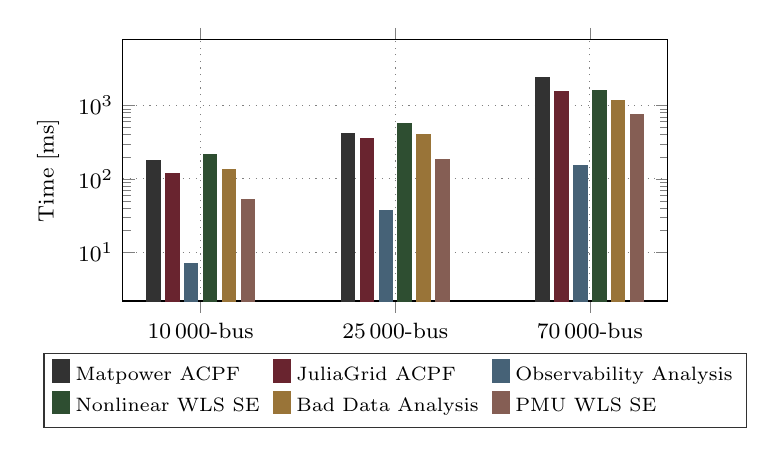
\begin{tikzpicture}
        \begin{axis}[
            ybar, 
            ymode=log,
            bar width = 0.17cm,
            symbolic x coords = {10\,000-bus, 25\,000-bus, 70\,000-bus},
            xtick=data,
            ylabel={Time [ms]},
            xlabel={Number of Buses},
            ytick = {10^1, 10^2, 10^3},
            enlargelimits=0.2,
  	    grid=major,   		
  	    width=8.5cm,height=4.9cm,
  	    tick label style={font=\footnotesize}, 
            label style={font=\footnotesize},
  	    legend style={at={(0.5,-0.20)}, align=left, 
            anchor=north,legend columns=3, font=\scriptsize, legend cell align=left},
            {/tikz/column 2/.append style={column sep=0.1cm}},
            {/tikz/column 4/.append style={column sep=0.1cm}},
            ]
            % matpower power flow
            \addplot[fill,black] coordinates {(10\,000-bus,177.4) (25\,000-bus,408) (70\,000-bus, 2433.9)};
            % juliagrid power flow
            \addplot[fill,richburgundy] coordinates {(10\,000-bus,116.8) (25\,000-bus,358.9) (70\,000-bus, 1539.9)};
            % observability 
            \addplot[fill,steelblue] coordinates {(10\,000-bus, 7) (25\,000-bus,37.23) (70\,000-bus, 150.8)};
            % nonlinear SE 
            \addplot[fill,forestgreen] coordinates { (10\,000-bus,215.5) (25\,000-bus,567.9) (70\,000-bus,1614.9)};
            % bad data analysis
            \addplot[fill,goldenrod] coordinates {(10\,000-bus,133.9) (25\,000-bus,402.9) (70\,000-bus,1169.2)};
            % PMU WLS SE
            \addplot[fill,rosybrown] coordinates {(10\,000-bus, 52.7) (25\,000-bus, 183.9) (70\,000-bus, 744.2)};

            \legend{
                \strut Matpower ACPF, \strut JuliaGrid ACPF, 
                \strut Observability Analysis, \strut Nonlinear WLS SE, \strut Bad Data Analysis,
                \strut PMU WLS SE
            }
        \end{axis}
    \end{tikzpicture}
    \caption{The execution times for ACPF solved using {\scalebox{0.85}{MATPOWER}} and JuliaGrid, observability analysis, nonlinear WLS SE followed by bad data analysis, and linear WLS SE using PMUs only with correlated measurement errors. Results are presented for power systems with 10\,000, 25\,000, and 70\,000 buses.}
    \label{plot1}
\end{figure} 

We use the {\scalebox{0.85}{MATPOWER}} ACPF execution times as benchmark values across all power systems to demonstrate that all analyses performed using JuliaGrid yield comparable execution times.
Although JuliaGrid achieves faster ACPF execution times, such as converging in 1539.9\,ms for a 70\,000-bus system compared to 2433.9\,ms with {\scalebox{0.85}{MATPOWER}}, the difference remain negligible. This similarity arises because both rely on operations like matrix factorizations and forward-backward substitutions, managed by basic linear algebra subprograms. However, JuliaGrid gains an advantage through in-place factorizations and the efficient formation of Jacobian matrices using fast for-loops, which are not directly replicable in {\scalebox{0.85}{MATLAB}}.

For the observability analysis, distinct randomly placed measurement sets are used for each power system, resulting in an average of seven maximal observable islands. The reported execution times include the identification of observable islands and also the restoration. To ensure a complete evaluation, the worst-case scenario is considered by using the largest pseudo-measurement set encompassing all possible measurements.

In the nonlinear WLS SE, the average number of measurements is 82\,948, 209\,504, and 577\,242 for power systems with 10\,000, 25\,000, and 70\,000 buses, respectively. For all cases the initial voltage values are taken from the power system's input data. These results demonstrate JuliaGrid's capability to solve SE problems efficiently for large-scale power systems. 

Followed by the solution from the nonlinear WLS SE, bad data analysis is performed. The reported execution times include both the detection and measurement removal processes. JuliaGrid's capability to handle the computational complexity of the normalized residual test stems from leveraging sparse inverse functions to retrieve only the necessary elements required for identifying bad data. For example, for the 70\,000-bus power system, JuliaGrid processed 577\,242 measurements to identify the largest normalized residual value in 1169.2\,ms.

Finally, we perform linear SE with PMUs only, with correlated measurement errors resulting in a non-diagonal covariance matrix. The number of measurements ranges from 53\,640 for the 10\,000-bus to 372\,365 for the 70\,000-bus power system. Despite the added complexity due to introduction of the non-diagonal covariance matrix, JuliaGrid demonstrates its capability to efficiently handle these analyses.

\subsection{Quasi-Steady-State Analyses}
Next, for the second set of experiments, we assess JuliaGrid's efficiency in solving quasi-steady-state analyses. In the first experiment we focus on DC model by solving PF and SE, while in the second experiment we evaluate PF and nonlinear SE related to AC model. We evaluate experiments for two time steps for power systems with 10\,000 and 70\,000 buses.
\begin{figure}[ht]
    \centering 
    \captionsetup[subfigure]{oneside,margin={1.4cm,0cm}}
    \begin{tabular}{@{\hspace{-0.5cm}}c@{}} 
    \subfloat[]{\label{plot2a} \centering	
        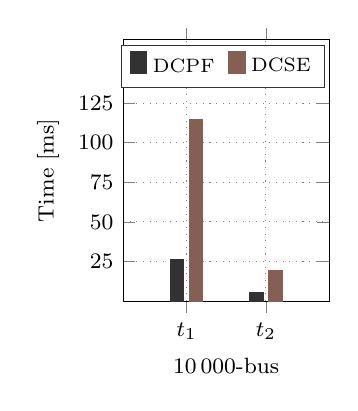
\begin{tikzpicture}
	    \begin{axis} [
                ybar, 
                bar width=0.17cm,
                symbolic x coords={$t_1$, $t_2$},
                xtick=data,
                ylabel={Time [ms]},
                xlabel={10\,000-bus},
                ytick = {25, 50, 75, 100, 125},
                ymin = 0,
                ymax = 165,
                enlargelimits=0.8,
                enlarge y limits=0,
      	    grid=major,   		
      	    width=4.2cm,height=4.9cm,
                log ticks with fixed point,
      	    tick label style={font=\footnotesize}, 
                label style = {font=\footnotesize, /pgf/number format/fixed},
      	    legend style={align=left, legend columns=2
                anchor=north, font=\scriptsize, legend cell align=left},
                {/tikz/column 2/.append style={column sep=0.1cm}},
                {/tikz/column 4/.append style={column sep=0.1cm}},
                ] 
                \addplot[fill,black] coordinates {($t_1$, 26.1) ($t_2$, 5.2)};
                \addplot[fill,rosybrown] coordinates {($t_1$, 114.7) ($t_2$, 19.2)};
                \legend{\strut DCPF, DCSE}    
            \end{axis}
	\end{tikzpicture}}
	\end{tabular}
	\captionsetup[subfigure]{oneside,margin={1.4cm,0cm}}
	\begin{tabular}{@{\hspace{0.3cm}}c@{\hspace{0cm}}} \subfloat[]{\label{plot2b} \centering	
        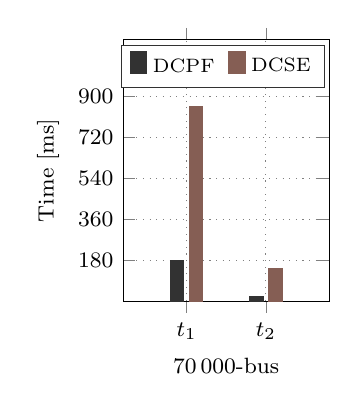
\begin{tikzpicture}
	    \begin{axis} [
                ybar, 
                bar width=0.17cm,
                symbolic x coords={$t_1$, $t_2$},
                xtick=data,
                ylabel={Time [ms]},
                xlabel={70\,000-bus},
                ytick = {180, 360, 540, 720, 900},
                ymin = 0.0,
                ymax = 1150,
                enlargelimits=0.8,
                enlarge y limits=0,
      	    grid=major,   		
      	    width=4.2cm,height=4.9cm,
                log ticks with fixed point,
      	    tick label style={font=\footnotesize, /pgf/number format/.cd, set thousands separator={},fixed}, 
                label style= {font=\footnotesize, /pgf/number format/fixed},
                legend style={align=left, legend columns=2
                anchor=north, font=\scriptsize, legend cell align=left},
                {/tikz/column 2/.append style={column sep=0.1cm}},
                {/tikz/column 4/.append style={column sep=0.1cm}},
                ]
                \addplot[fill,black] coordinates {($t_1$, 179.8) ($t_2$, 20.7)};
                \addplot[fill,rosybrown] coordinates {($t_1$, 858.1) ($t_2$, 143.7)};
                \legend{\strut DCPF, DCSE}    
            \end{axis}
	\end{tikzpicture}}
	\end{tabular}
        \caption{The execution times for quasi-steady-state analyses, including DCPF and DCSE, for a 10\,000-bus power system (subfigure a) and a 70\,000-bus power system (subfigure b) over time steps $t_1$ and $t_2$.}
	\label{plot2}
\end{figure} 

For the first experiment, the DCPF model is generated and solved, with the nodal admittance matrix factorization being the primary computational task. Based on the DCPF results, a measurement model is created, incorporating active power flows at both ends of all branches and injection measurements at all buses. This measurement model is used to formulate and solve the DCSE. As shown in \figurename~\ref{plot2}, the total time for $t_1$ includes the DCPF solving time as well as the loading time for power system data from HDF5 file. For the DCSE, the time includes both solving the DCSE and generating the measurement set using JuliaGrid's built-in functions. Note that the generation of measurement set forms a significant portion of the total time\footnote{The measurement model in DCPF is built using functions that add measurements individually, which is less efficient than generating complete sets as in AC analyses. This feature is excluded for DC analyses since AC-based measurements better represent real system conditions.}.



For the time step $t_2$, we randomly modify 20\% of the generator outputs and load values. JuliaGrid's built-in functions facilitate simultaneous updates to the power system data and the DCPF model, followed by re-solving of DCPF. The DCPF execution time in this step is significantly lower because JuliaGrid reuses the previously factored nodal admittance matrix. Note that the reported time also includes the time required to update the power system data and the DCPF model. For the updated power system, a new measurement set reflecting the changes is required. However, instead of creating a new measurement model, the previously defined model is updated together with the DCSE model. This approach significantly reduces the execution time for the DCSE by reusing both the measurement model and the gain matrix factorization. This demonstrates that JuliaGrid can significantly reduce execution time for specific scenarios, particularly when the nodal admittance or gain matrix remains unchanged across time steps. 

A similar conclusion holds for the AC model when only loads and generator outputs are altered. In this case, the fast Newton-Raphson method can be employed, where factorized matrices are reused in each subsequent step, significantly reducing the time required to construct a measurement model. 

In the second experiment, we demonstrate that JuliaGrid can reduce execution times after the initial step, even in scenarios where factorized matrices cannot be reused. The time reduction is a juxtaposition of the different approaches, such as reusing formed vectors, matrices, and using in-place factorizations. In addition, for all non-linear algorithms JuliaGrid automatically initiates a warm start for each new sequence. Let us solve ACPF using the Newton-Raphson method and the nonlinear SE using the Gauss-Newton method for power systems with 10\,000 and 70\,000 buses. As shown in \figurename~\ref{plot2} for the first time step $t_1$, the time for ACPF includes the loading time of the power system data with the time needed to create the AC model, and convergence time. Using results from ACPF, we generate the measurement set and solve the nonlinear SE to obtain the WLS estimator, which gives the execution time for WLS SE. Note that the number of measurements is 32\,283 and 224\,539 for power systems with 10\,000 and 70\,000 buses, respectively. 
\begin{figure}[ht]
    \centering 
    \captionsetup[subfigure]{oneside,margin={1.4cm,0cm}}
    \begin{tabular}{@{\hspace{-0.5cm}}c@{}} 
    \subfloat[]{\label{plot3a} \centering	
        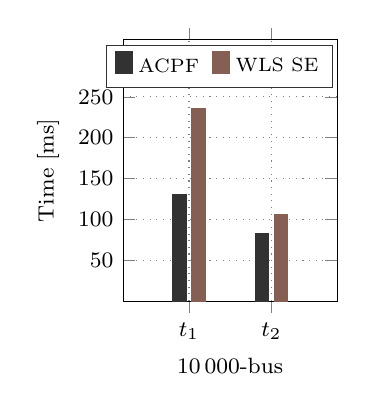
\begin{tikzpicture}
	    \begin{axis} [
                ybar, 
                bar width=0.17cm,
                symbolic x coords={$t_1$, $t_2$},
                xtick=data,
                ylabel={Time [ms]},
                xlabel={10\,000-bus},
                ytick = {50, 100, 150, 200, 250},
                ymin = 0,
                ymax = 320,
                enlargelimits=0.8,
                enlarge y limits=0,
      	    grid=major,   		
      	    width=4.3cm,height=4.9cm,
                log ticks with fixed point,
      	    tick label style={font=\footnotesize}, 
                label style = {font=\footnotesize, /pgf/number format/fixed},
      	    legend style={align=left, legend columns=2
                anchor=north, font=\scriptsize, legend cell align=left},
                {/tikz/column 2/.append style={column sep=0.1cm}},
                {/tikz/column 4/.append style={column sep=0.1cm}},
                ]
                \addplot[fill,black] coordinates {($t_1$, 130.5) ($t_2$, 82.6)};
                \addplot[fill,rosybrown] coordinates {($t_1$, 235.8) ($t_2$, 105.5)};
                \legend{\strut ACPF, WLS SE}   
            \end{axis}
	\end{tikzpicture}}
	\end{tabular}
	\captionsetup[subfigure]{oneside,margin={1.6cm,0cm}}
	\begin{tabular}{@{\hspace{0.3cm}}c@{\hspace{0cm}}} \subfloat[]{\label{plot3b} \centering	
        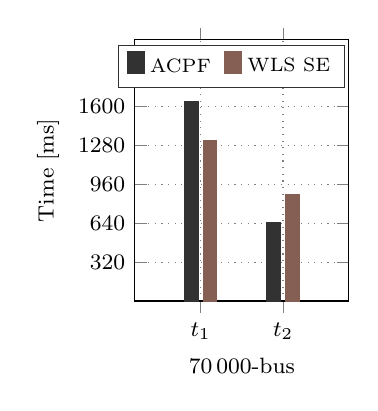
\begin{tikzpicture}
	    \begin{axis} [
                ybar, 
                bar width=0.17cm,
                symbolic x coords={$t_1$, $t_2$},
                xtick=data,
                ylabel={Time [ms]},
                xlabel={70\,000-bus},
                ytick = {320, 640, 960, 1280, 1600},
                ymin = 0.5,
                ymax = 2150,
                enlargelimits=0.8,
                enlarge y limits=0,
      	    grid=major,   		
      	    width=4.3cm,height=4.9cm,
                log ticks with fixed point,
      	    tick label style={font=\footnotesize, /pgf/number format/.cd, set thousands separator={},fixed}, 
                label style= {font=\footnotesize, /pgf/number format/fixed},
                legend style={align=left, legend columns=2
                anchor=north, font=\scriptsize, legend cell align=left},
                {/tikz/column 2/.append style={column sep=0.1cm}},
                {/tikz/column 4/.append style={column sep=0.1cm}},
                ]
                \addplot[fill,black] coordinates {($t_1$, 1639.9) ($t_2$, 644.4)};
                \addplot[fill,rosybrown] coordinates {($t_1$, 1318.5) ($t_2$, 875.7)};
                \legend{\strut ACPF, WLS SE} 
            \end{axis}
	\end{tikzpicture}}
	\end{tabular}
        \caption{The execution times for quasi-steady-state analyses, including ACPF and nonlinear WLS SE, for a 10\,000-bus power system (subfigure a) and a 70\,000-bus power system (subfigure b) over time steps $t_1$ and $t_2$.}
	\label{plot3}
\end{figure} 

Next, we modify the off-nominal turn ratio of all transformers in the system by ±1\% followed by re-solving the ACPF. To achieve this modification, we update both the power system data and the ACPF model using built-in functions. This update allows us to reuse the AC model, the Jacobian matrix pattern, and run the Newton-Raphson method in a warm start, leading to a reduced execution time for time step $t_2$. We update the previous measurement model, along with the nonlinear WLS SE model. This results in reusing the patterns of the measurement vector, Jacobian matrix, and the covariance matrix. Additionally, the Gauss-Newton method is automatically initialized in a warm start. This synergy of techniques results in faster execution time for the step $t_2$.

\section{Conclusions}
This paper presents the JuliaGrid, an open-source framework, implemented in the Julia programming language. The majority of the JuliaGrid's codebase represents the independent implementation, minimizing reliance on external packages beyond Julia’s standard library. This approach ensures long-term support for algorithms integrated within the framework. JuliaGrid is optimized for solving large-scale problems in PF, OPF, observability analysis, SE algorithms, and bad data analysis. The framework's architecture centres around code-reusability paradigm, allowing creation of power system models including AC and DC models and measurement models. These models can be combined independently for the design of new user-defined algorithms. To simplify the learning curve for both utilizing existing functionalities and designing new algorithms, JuliaGrid offers comprehensive documentation and a rich repository of examples, making it an invaluable resource for the educational and research communities.

\bibliographystyle{IEEEtran}
\bibliography{cite}

\end{document}